% ai-phishing-detection-dissertation/report/sections/4-results/distilbert-model-performance/performance-on-independent-test-sets.tex

\subsubsection*{Performance on independent test sets}
The DistilBERT model's generalisation ability is tested against the same independent data sources as the Random Forest model was. Performance on these datasets are detailed in the table below. Confusion matrices are also subsequently presented.

\begin{table}[h]
\centering
\begin{tabularx}{\textwidth}{|X|X|X|X|X|X|}
\hline
\textbf{Dataset} & \textbf{Accuracy} & \textbf{Precision (Phish)} & \textbf{Recall (Phish)} & \textbf{F1-Score (Phish)} & \textbf{ROC AUC} \\
\hline
SpamAssassin Easy Ham & \texttt{0.9584} & \texttt{0.0000} & \texttt{0.0000} & \texttt{0.0000} & \texttt{NaN} \\
\hline
SpamAssassin Hard Ham & \texttt{0.9880} & \texttt{0.0000} & \texttt{0.0000} & \texttt{0.0000} & \texttt{NaN} \\
\hline
Nigerian Fraud Test & \texttt{0.3175} & \texttt{1.0000} & \texttt{0.3175} & \texttt{0.4820} & \texttt{NaN} \\
\hline
Nazario Phishing Test & \texttt{0.3773} & \texttt{1.0000} & \texttt{0.3773} & \texttt{0.5479} & \texttt{NaN} \\
\hline
SpamAssassin Spam/Phish (Test Portion) & \texttt{0.2827} & \texttt{1.0000} & \texttt{0.2827} & \texttt{0.4408} & \texttt{NaN} \\
\hline
\end{tabularx}
\caption{DistilBERT model performance on independent test sets}
\end{table}

\begin{figure}[H]
  \begin{center}
    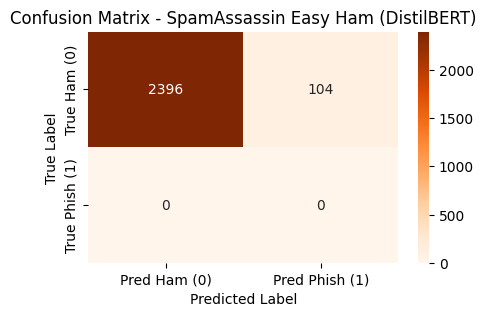
\includegraphics[scale=0.85]{confusion-matrices/distilbert/spamassassin-easy-ham.png}
    \caption{Confusion matrix for DistilBERT on SpamAssassin Easy Ham test set}
  \end{center}
\end{figure}

\begin{figure}[H]
  \begin{center}
    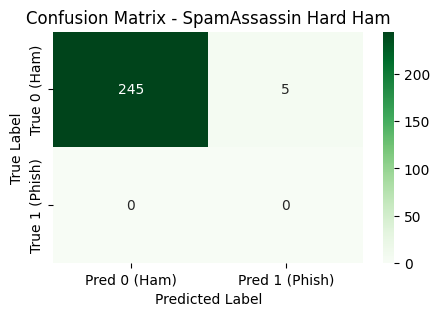
\includegraphics[scale=0.85]{confusion-matrices/distilbert/spamassassin-hard-ham.png}
    \caption{Confusion matrix for DistilBERT on SpamAssassin Hard Ham test set}
  \end{center}
\end{figure}

\begin{figure}[H]
  \begin{center}
    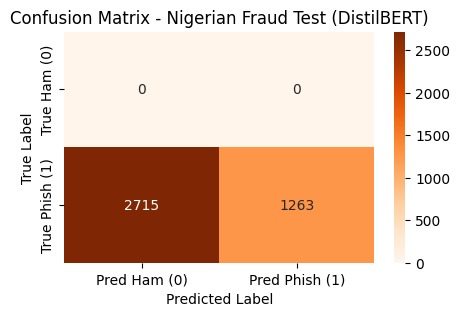
\includegraphics[scale=0.85]{confusion-matrices/distilbert/nigerian-fraud.png}
    \caption{Confusion matrix for DistilBERT on Nigerian Fraud test set}
  \end{center}
\end{figure}

\begin{figure}[H]
  \begin{center}
    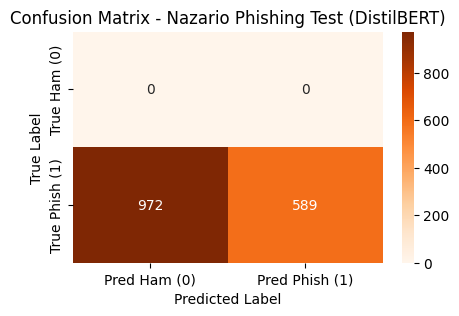
\includegraphics[scale=0.85]{confusion-matrices/distilbert/nazario-spam.png}
    \caption{Confusion matrix for DistilBERT on Nazario Spam test set}
  \end{center}
\end{figure}

\begin{figure}[H]
  \begin{center}
    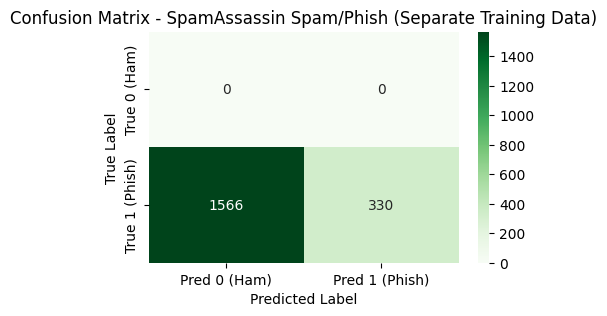
\includegraphics[scale=0.85]{confusion-matrices/distilbert/spamassassin-additional.png}
    \caption{Confusion matrix for DistilBERT on an additional SpamAssassin test set}
  \end{center}
\end{figure}

\noindent As seen with the Random Forest model, the DistilBERT model showed high accuracy with the SpamAssassin "ham" datasets with complete correct predictions for each instance. Evaluation on independent, external datasets show a significant drop in recall for the phishing class, ranging from values of 0.2827 to 0.3773, but did remain perfect for phishing instances. Like before, there is a strong performance with in-distribution test data, and ROC AUC score can not be calculated for these evaluations.
